\section{Folding crease patterns} \label{sec:folding}
In this section we explore the different ways one can fold a given crease pattern. Our result is a discrete combinatorial charecterization for the local existence of a fold along a piecewise DOG.

\begin{figure} [h]
	\centering
	\includegraphics[width=0.7\linewidth]{figures/curved_fold_through_curve.pdf}
	\caption{(TODO BETTER FIG Computation and then maybe Katja) In the future I'll place here a crease pattern and 4 different configuration for the same deformation of the curve. 2 of them will be 2 different smooth surfaces and the other two will be curved folds by picking 2 different ones from both sides. }
	\label{fig:folding_combinatorics}
\end{figure}

%Two intersecting developable surfaces can be flattened along their intersection if the intersected curve have the same geodesic curvature on both surfaces. 
\subsection{The smooth and combinatorial parameters around a single curve crease}
Straight creases are rather boring, mathematically speaking. Straight lines can only be folded as in classical origami, i.e. by keeping them straight \cite{demaine_lens}. Hence a folding of a single straight crease can be described by a single real number, representing the constant dihedral angle between the nearby planes. There are far more ways, i.e. degrees of freedom, to fold of a curved crease; Up to rigid motion, a curved folded surface can locally be described by two smooth \textit{functions}: the curves' curvature $k(t) > k_g(t)$ and its torsion $\tau(t)$  \cite{more_on_paper, duncan_folded}. Indeed, let $\gamma(t)$ be a curve on a flattened crease pattern and $\Gamma(t)$ is its embedding in $\mathbb{R}^3$. Let $k(t)$ be the curvature of $\Gamma(t)$, and $k_g(t)$ the curvature of of $\gamma(t)$, i.e. the curve's geodesic curvature, such that $k_g(t) = k(t) \cos(\alpha(t))$. Assuming the curve along the surface is indeed bend such that $k(t) > k_g(t)$, then there are 2 distinct planes containing $\Gamma'(t)$ and forming an angle of $\alpha(t)$ with the curve's osculating plane. A curve folded surface is then a consistent smooth choice of a different tangent plane for each "side" of the curve, which are dependent on $k(t),\tau(t)$ (see Fig. \ref{fig:folding_combinatorics}). The angle between the different surfaces tangent planes along the curve is said to be the folding angle, which generally does change along the curve, and is bisected by the osculating plane of the curve \cite{curved_folding_kilian,more_on_paper,duncan_folded}. The ruling patterns of the surfaces change as well during the deformation, making modeling of such surfaces using discrete ruling based challenging  (see \figref{fig:rulings_problem_curve}). Thus changing the curves' curvature and torsion, dictates the shape of the surface in its surrounding, where ruling emanating from the curve continue globally until the surfaces' boundary. The folded shape is locally not determined only by these two smooth functions as there is an additional \textit{combinatorial} degree of freedom: the choice of a surface at each side (see \figref{fig:folding_combinatorics}). Assuming a given flat curve on a developable surface is deformed to lie in $R^3$ and the two patches around it stays $C^2$ then there are locally four possible configurations for a developable surfaces passing through it: two of which creates discontinuity along the crease, meaning a curved folded surface (see \figref{fig:folding_combinatorics}). %We call one folded configuration a mountain fold and the other a valley fold. %We follow \cite{demaine_lens} to distinguish between the two type of folded configurations by calling one choice a \textit{Mountain} fold and the other a \textit{Valley} fold. %We note that by \cite{demaine_lens}, a fold always consistently stays mountain/valley throughout the entire creased curve. Assuming a given normal orientation, a fold is said to be a mountain fold if the normal of the surface TODO:ADD EXPLANATION. 


%The curvature and torsion also dictates the ruling patterns of the developable surfaces, generally changing while folding and bending the surface. Deforming a curved crease locally determines the shape of both surfaces around it, and the exact regions of surfaces influenced by that fold depend on the ruling patterns themselves. As mentioned, the rulings patterns themselves can change which can smoothly change during the deformation itself. 

%(there's the cone singularity case where a curved fold is more local (as focused on the cone point) but I think this requires the curve to be C^1.. should mention it?

\subsection{The combinatorial parameters of multiple creases}
The previous analysis explains the local behaviour of curved folding around a small part of a single curve, as the reflection of tangent planes along the curve osculating plane. Understanding crease patterns globally still remains a challenge. In essence, deforming one patch propagates a global deformation of the patch on the other side of the crease, a process that depends on the fixed creases and the possibly changing ruling patterns. When there are multiple creases this process further propagate and dictates the shape of other patches The process becomes more complicated when some creases intersect due to compatibility constraints (see \figref{fig:multiple_crease_patterns}). 

\begin{figure} [h]
	\centering
	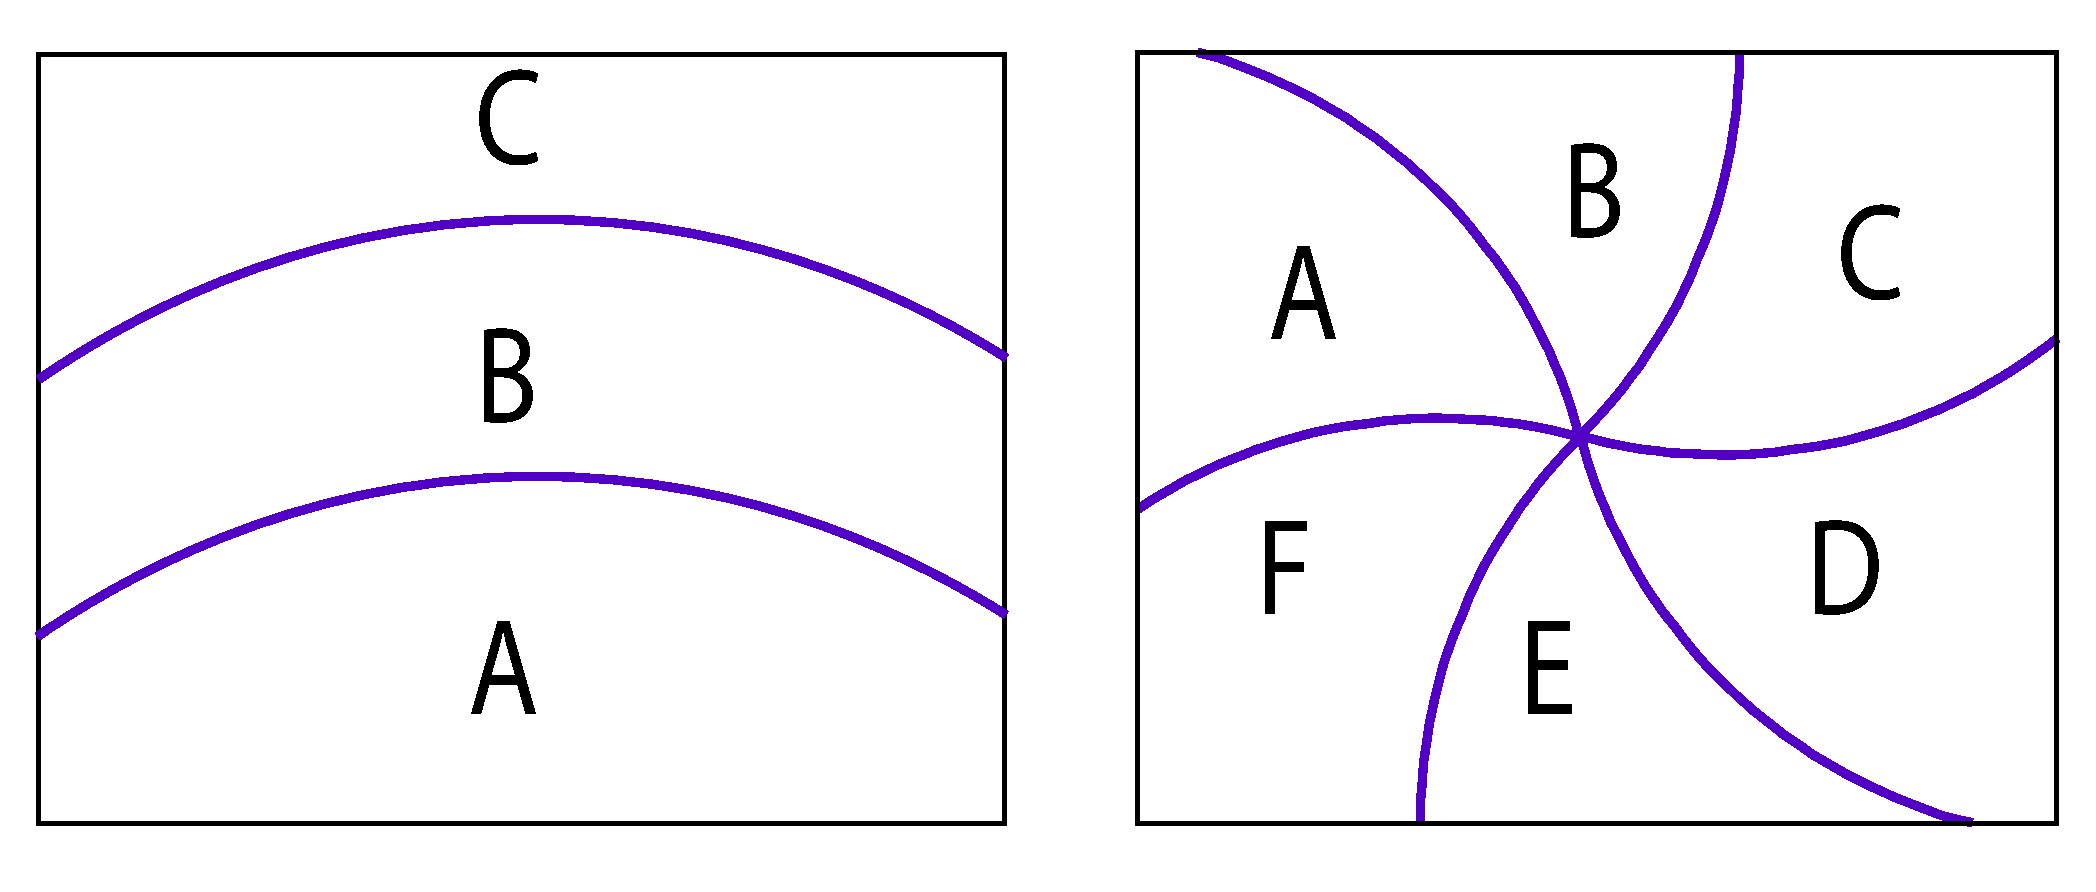
\includegraphics[width=0.7\linewidth]{figures/multiple_crease_patterns}
	\caption{\MiR{Todo caption: propagation of constraints from A to B to C, and a star.}}
	\label{fig:multiple_crease_patterns}
\end{figure}

Generally speaking, one might be able to choose between 4 configurations of the surface at the first crease, but this choice already fixes a patch for nearby creases. The combinatorial degrees of freedom that then remain are whether each crease is folded or not (see \figref{fig:folded_and_not_folded} ). With this in mind, we note the following observation:

\begin{theorem}\label{Thm:supporting_plane}
A crease curve is folded along a given point if and only if its osculating plane at that point is locally a supporting plane for the surface (see \figref{fig:plane_side}).
\end{theorem}

\begin{figure} [h]
	\centering
	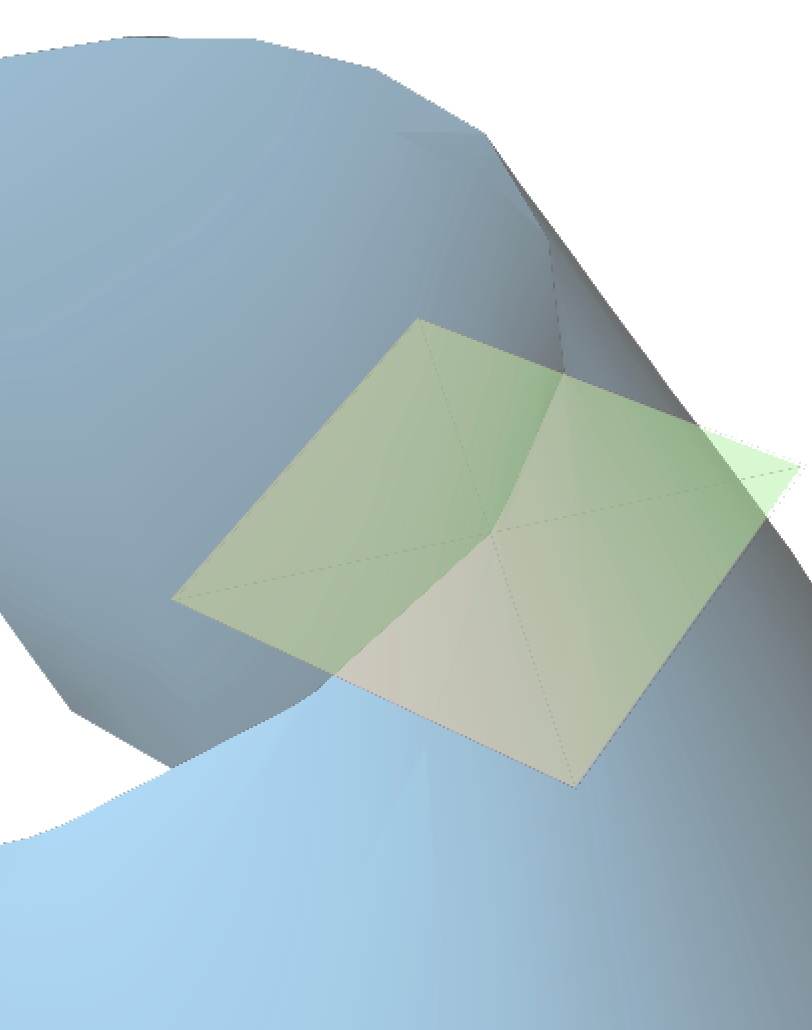
\includegraphics[width=0.5\linewidth]{figures/plane_side}
	\caption{\MiR{TODO: caption and better figure}}
	\label{fig:plane_side}
\end{figure}

This follows directly from the fact that the tangent planes along a crease are the same if it is smooth along it, but along a folded crease they are reflections of one another through the curve's osculating plane. %We also note that when the curvature of the curve is not larger than its geodesic curvature, one example being a flat patch, then the tangents from both sides are the same (we should maybe call it both active and not active for that configuration?


% Motivated by homotopy stuff, we look for a function F(t). Once a crease is active, there's no need to take care of it.

% The pictures which will show are then discrete, though the smooth picture is the same. Maybe put the discrete picture in the setup as well.
% A fold is active if nearby tangents are reflections of one another, and is not active if they are the same as there is no discontinuity. (have a figure that is discrete, but explain it is also the same drawing for the smooth case).
% Write down the formula. Write down a flow. State it is inequality hence folding should be done at time = 0 when it is flat, but nevertheless a binary decision. We characterize it by the sign. 
% One can then view a folding-bending process as a smooth flow, i.e. a smooth deformation on a piecewise C^2 developable surface. The choice to make each fold active is only done during time t = 0, whereas otherwise discontinuties arise, and locally remains a curved fold as the equality.
% Problem in using it for a DOG is that we cannot hope to get it exactly. Then present binary representation. Say how it's really good (also goes to zero very fast).
% The binary characterization in the smooth case, motivate more degrees of freedom, and add the algorithm. Then add control for dihedral angles and mountain valley fold.

\subsection{Discretization}
We discretize the condition by constraining tangents formed by the orthogonal grid parameter lines to lie on one side of the curve's discrete osculating plane (see \figref{fig:osc_plane_discretization} for the notations of the edges). The edges intersecting the crease can be considered as discrete tangents originating at crease points. In the notation of \figref{fig:osc_plane_discretization}, each connected component has its own edge $e^1,e^2$ intersecting the crease. At a starting flat configuration they are the same, but a folding movement creates a discontinuity along them. We denote the tangents as $t_1 = \frac{t_1}{\|t_1\|}, t_2 = \frac{t_2}{\|t_2\|}$. We denote the curves binormal, i.e. its osculating plane's normal as $B = \frac{e_f \times e_b}{\|e_f \times e_b\|}$, noting that $e_f,e_b$ are the same along both connected components.

\begin{figure} [h]
	\centering
	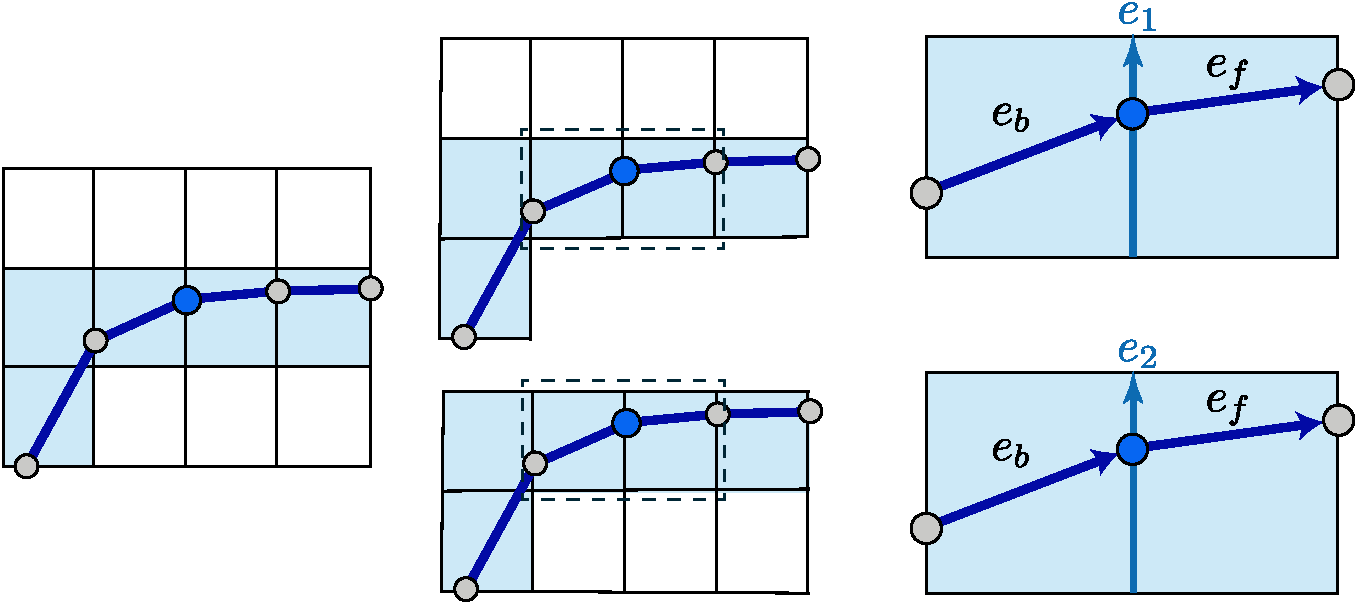
\includegraphics[width=\linewidth]{figures/osc_plane_discretization}
	\caption{Notation for edges along a crease pattern. Left: An orthogonal grid with a crease curve. Center: Following \cite{rabi2018shape}, we represent such a part by duplicating quads along the grid, creating different connected components while positionally constraining the curve edge points to match. Right: Notation for a duplicated edge intersecting the curve at the blue points ($e_1,e_2$), and the forward and backwards crease edges at the blue points ($e_f,e_b$). }
	\label{fig:osc_plane_discretization}
\end{figure}

In the notation of \figref{fig:osc_plane_discretization}, this constraint can be written as:
\begin{equation} \label{eq:folding_const_normalized} 
\text{sgn}(\langle t^1,B\rangle) +  {sgn}(\langle t^2,B\rangle) = 0
\end{equation}
with 
\begin{equation} \label{eq:sign}
\text{sgn}(x) = \left\{
     \begin{array}{@{}l@{\thinspace}l}
       -1  &: \text{if } x < 0, \\
       0 &: \text{if } x = 0, \\
       1 &: \text{if } x > 0. \\
     \end{array}
   \right.
\end{equation}

%There is in fact no need to normalize the tangents and binormal directions, as the following constraint is equivalent to \eqref{eq:folding_const_normalized}:
%\begin{equation} \label{eq:folding_const}
%\text{sgn}(\langle e^1,e_f \times e_b \rangle) +  {sgn}(\langle e^2,e_f \times e_b\rangle) = 0
%\end{equation}

%\begin{equation} \label{eq:folding_const}
%\text{sgn}(\langle e^1,e_f \times e_b \rangle) +  {sgn}(\langle e^2,e_f \times e_b\rangle) = 0
%\end{equation}

\subsection{Discussion}
There are multiple equivalent charecterizations for a folded crease over a curved folded surface. We would like to point out some key properties of our chosen discretization for the constraint, i.e. \eqref{eq:folding_const_normalized}, and briefly discuss how these are not satisfied by different constraint choices. \\
\textbf{It is suitable for homotopy based optimization methods} as it is satisfied on a flat mesh. In this sense we consider a point along a curve with zero normal curvature as both folded and not folded. \\ 
\textbf{It is minimal} and generally non-intrusive. Once a curved crease is folded on a piecewise smooth developable surface, one does not need to explicitly take extra care of folding. The effect of eq. \eqref{eq:folding_const} on an already-folded surface is null. The discontinuity along the tangents caused by the folding implies that a folded crease remain folded under local deformations, and in order for it to become unfolded one need to first flatten it, as this is the case for a piecewise smooth curved folded surface. It also captures the converse: a curved crease can only be folded from a point with zero normal curvature \cite{more_on_paper}. \\
One could for instance distinguish curved folded with non-curved folded configurations using discontinuties along the tangents $t_1,t_2$, but lose the feasibility of the flat models. Moreover, in the discrete case a minor discontinuity can still arise even though there is no fold, i.e. where eq. \eqref{eq:folding_const_normalized} is not satisfied, thus numerically giving the impression of a fold when visually there is none. Another option is to define folded configurations as those satisfying the similar but simpler smooth constraint:
\begin{equation} \label{eq:folding_const_smooth} 
\langle t^1,B\rangle + \langle t^2,B\rangle = 0
\end{equation}
This condition is satisfied exactly in flat models and in any piecewise smooth curved folded surface as tangent planes along a folded creased curve are reflections of one another in the osculating plane of the curve. However, the conditions are not satisfied \emph{exactly} on every folded piecewise DOG (as evident by all models in this paper). An exception to this is the class of curved crease with zero torsion, in which case the folds are simply formed as a global plane reflection \cite{Mitani_ref}. Therefore, enforcing constraint \eqref{eq:folding_const_smooth} as a hard constraint is too restrictive in practice, while enforcing it as a soft constraint creates a constraint that unlike the smooth case, does not vanish once a crease is folded and hence is not minimal.

\section{Folding angles and mountain-valley assignments} \label{sec:folding_angles_mountain_valley}
To allow a designer more expressiveness and freedom we show how to constrain the folding angles around folds, i.e. the angle between the tangent planes around a crease. This can be done by simply constraining tangents around the fold; A folding deformation can be seen as a rotation of tangent vectors around a crease vertex tangent. On a straight fold, the crease tangent is constant and so is the folding angle, while around a curved crease both are generally changing. If the folding angle is $\theta$, then tangents on both sides that are orthogonal to the crease tangent form an angle of $\theta$, while tangents that are parallel to the crease pattern remain parallel to each other. The following lemma shows the relation between an angle of tangents that are equal on a flat configuration and the folding angle: 
 \begin{lemma}  \label{lem:laplace_cheb}
 Let $t_1,t_2$ be tangents on two sides of a crease curve at a given point that are equal on the flattened isometric developable surface. Let $t$ be the crease curve tangent. Assuming the surface went through a curved folding isometric deformation and the folding angle at a given point along the crease is $\theta$ then the tangents satisfy:
\begin{equation}
\langle t_1, t_2 \rangle = cos(\alpha)^2 + sin^2(\alpha) cos(\theta) \end{equation}
%4*cos(alpha/2)/(norm(e1)+norm(e2))
\end{lemma}
\begin{proof}{Let $\{t,n,b\}$ be the Frenet frame of the curved crease. An angle $\alpha$ means that at the flat isometric configuration both tangents can be written as $cos(\alpha)t + sin(\alpha)n$. A folding angle of $\theta$ at a given point means that relative to the Frenet frame of the curve, tangents on one surface where rotated in angle $\frac{\theta}{2}$ around the crease's tangent $t$, while on the other surface they were rotated in an angle  $-\frac{\theta}{2}$. Thus w.l.o.g $t_1 = cos(\alpha)t + sin(\alpha)(cos(\frac{\theta}{2})n+sin(\frac{\theta}{2})b)$ and $t_2 = cos(\alpha)t + sin(\alpha)(cos(\frac{\theta}{2})n-sin(\frac{\theta}{2})b)$. The proof ends by computing $\langle t_1,t_2 \rangle$ and plugging in the trigonometric identity $cos(\theta) = cos^2(\frac{\theta}{2})-sin^2(\frac{\theta}{2})$.}\end{proof}

\MiR{add figure for dihedral fold and for M/V assignment}

As mentioned, there is sometimes an extra combinatorial degree of freedom in choosing the type of fold, i.e. the choice of surfaces from each side of the curve (see \figref{fig:folding_combinatorics}). We follow \cite{demaine_lens} to distinguish between the two type of folded configurations by calling one choice a \textit{Mountain} fold and the other a \textit{Valley} fold. We would like to emphasis that for straight folds this degree of freedom always exists, but around curved creases it often doesn't. In fact, a common case on a curved crease pattern is that its possible to choose only one Mountain/Valley (M/V) assignment, were the rest are determined by the propagation of the rulings (\MiR{point to figure, should be better than I have now}), motivating us to look at the condition \eqref{eq:folding_const_normalized}. 

\MiR{Add above and below the tangent planes condition, and derivation by the sign of <t1,txt2> =<t2,t1xt>}